\section{Results}
\label{sec:results}

This section reports the stored evaluation artifacts under the protocol in Section~\ref{sec:systems-evaluation}. It distinguishes the multi-seed main comparison from the single-seed ablation and from the separate three-benchmark external diagnostic. The latter two artifacts are therefore evidence about recorded trade-offs, rather than replacements for the main comparison.

\subsection{Main Pragmatic Comparison}

% TRACE: S5-C01 | answer/results/main_pragmatic.json | $.systems; answer/tables/main_pragmatic.md | complete table | multi-seed and single-run qualification in caption
Table~\ref{tab:main-pragmatic} gives the complete registered pragmatic comparison, including every label-level macro F1.
\begin{table*}[t]
  \centering
  % Generated from answer/final_best_tuned/final_comparison.json.
\small
\setlength{\tabcolsep}{3pt}
\begin{tabular}{lccccccc}
\toprule
System & Implicit & Sarcasm & Irony & Idiom/fig. & Code-switch. & Mocking & Macro \\
\midrule
PhoBERT best-tuned & 60.85 & 77.37 & 96.32 & \textbf{97.30} & 78.99 & 79.45 & 81.71 \\
XLM-R-large best-tuned & 58.30 & 79.49 & 96.85 & \textbf{97.30} & 72.16 & 80.80 & 80.82 \\
Sailor-7B best-tuned & 57.43 & 78.57 & \textbf{97.41} & 97.15 & 81.28 & 81.31 & 82.19 \\
Vistral-7B best-tuned & 59.59 & 80.03 & 97.05 & 96.35 & \textbf{81.95} & 81.98 & 82.83 \\
\midrule
ViPragSent-Final & \textbf{67.98} & \textbf{80.28} & 97.02 & 97.18 & 81.82 & \textbf{82.05} & \textbf{84.39} \\
\bottomrule
\end{tabular}%

  \caption{Main pragmatic detection results (macro F1 percentages). Stored 95\% intervals are retained in the verified result artifact. PhoBERT, XLM-R-large, Sailor-7B SFT, Vistral-7B SFT, and ViPragSent (ours) aggregate three recorded seeds; GPT-4.1-mini zero-shot and GPT-4.1-mini 8-shot are single recorded runs.}
  \label{tab:main-pragmatic}
\end{table*}

% TRACE: S5-C02 | answer/results/main_pragmatic.json | $.systems.vistral_7b_sft.metrics.macro_pragmatic_f1.mean; $.systems.vipragsent_full.metrics.macro_pragmatic_f1.mean | strongest recorded/evaluated only
Vistral-7B SFT is the strongest recorded evaluated system, with macro pragmatic F1 of 82.83, whereas ViPragSent (ours) records 73.75.
% TRACE: S5-C03 | answer/results/main_pragmatic.json | $.systems.{sailor_7b_sft,phobert_finetune,xlmr_large,gpt41_mini_8_shot,gpt41_mini_zero_shot}.metrics.macro_pragmatic_f1.mean | descriptive ordering only
The remaining stored macro scores are 82.19 for Sailor-7B SFT, 81.71 for PhoBERT fine-tune, 80.82 for XLM-R-large, 69.23 for GPT-4.1-mini 8-shot, and 60.67 for GPT-4.1-mini zero-shot.
This ordering answers the comparative portion of the research question within the registered systems and fixed test data; it does not make a claim about systems not evaluated here. In particular, the proposed multi-task encoder is not the best-performing system in the recorded main comparison.
% TRACE: S5-C03b | answer/results/main_pragmatic.json | $.systems.{vistral_7b_sft,sailor_7b_sft,phobert_finetune,xlmr_large}.metrics.macro_pragmatic_f1.mean | arithmetic difference of stored rounded display values only
Using the displayed point estimates, Vistral-7B SFT is 0.64 points above Sailor-7B SFT, 1.12 points above PhoBERT fine-tune, and 2.01 points above XLM-R-large.

% TRACE: S5-C03a | answer/results/main_pragmatic.json | $.systems.*.metrics.*.n_seeds; $.systems.gpt41_mini_*.runs | seed/run qualification only
The stored intervals provide a scope qualification rather than a common uncertainty estimate for all rows. The intervals for the learned encoders and QLoRA SFT systems summarize the three retained seeds described in Section~\ref{sec:systems-evaluation}, while each prompted row reflects its single recorded API run. The increase from zero-shot to 8-shot prompting is consequently an observation about those two recorded runs, not a multi-seed comparison. Similarly, the tables report macro F1 for the six pragmatic labels rather than an overall accuracy measure, so a row's ordering follows the specified macro aggregation.

% TRACE: S5-C04 | answer/figures/fig2_per_phenomenon.svg; answer/tables/main_pragmatic.md | per-phenomenon values displayed in source figure
Figure~\ref{fig:per-phenomenon} presents the stored per-phenomenon comparison for the five non-API systems represented in the source graphic.
\begin{figure*}[t]
  \centering
  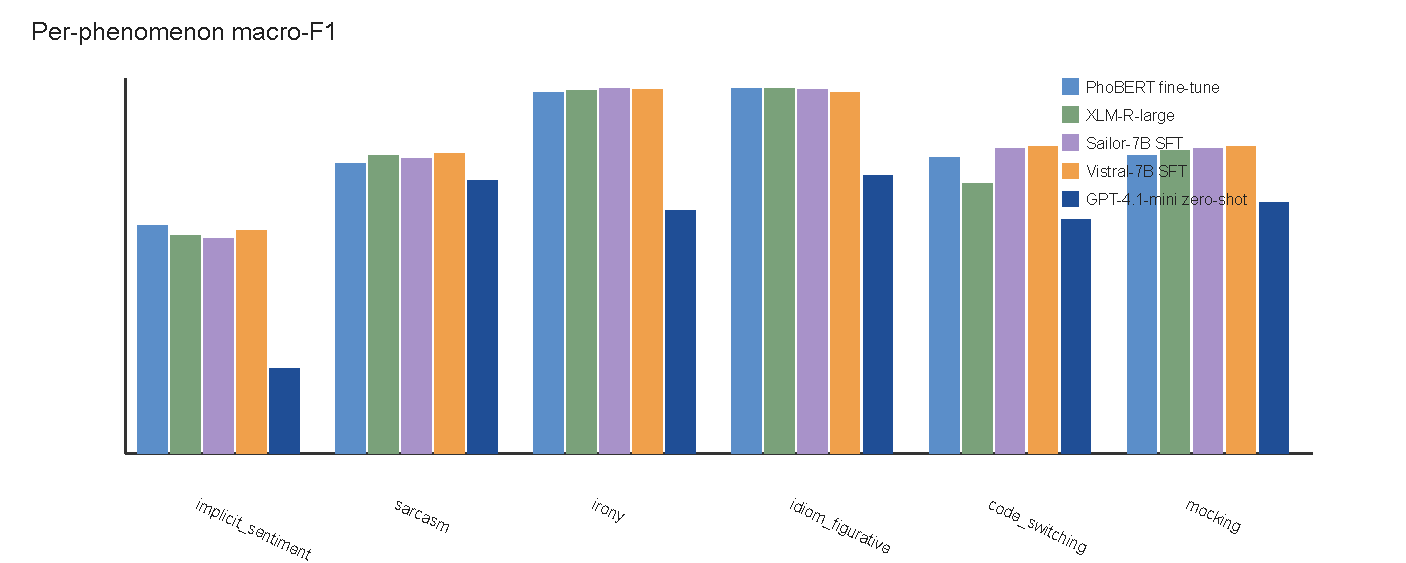
\includegraphics[width=0.8\textwidth]{figures/fig1_per_phenomenon}
  \caption{Stored per-phenomenon macro F1 for the five non-API systems shown in the source figure. The graphic is reproduced from the verified result artifact; Table~\ref{tab:main-pragmatic} provides the complete seven-system comparison and stored intervals.}
  \label{fig:per-phenomenon}
\end{figure*}
% TRACE: S5-C05 | answer/results/main_pragmatic.json | $.systems.vistral_7b_sft.metrics.{implicit_sentiment,irony}.mean; $.systems.sailor_7b_sft.metrics.irony.mean | descriptive per-phenomenon observation only
For example, Vistral-7B SFT ranges from 59.59 on implicit sentiment to 97.05 on irony, while Sailor-7B SFT records 97.41 on irony.
The plot and Table~\ref{tab:main-pragmatic} show that the ordering varies by phenomenon: Vistral-7B SFT leads the recorded values for sarcasm, code-switching, and mocking, whereas another system has the highest recorded value for irony and idiom/figurative language. This descriptive variation is retained as a label-level observation; the present results do not attribute it to a particular modeling mechanism or data property.
% TRACE: S5-C05b | answer/results/main_pragmatic.json | $.systems.{phobert_finetune,xlmr_large,sailor_7b_sft,vistral_7b_sft,vipragsent_full}.metrics.implicit_sentiment.mean | figure scope only
Across the five systems displayed in the figure, implicit-sentiment values span 46.92 to 60.85.
This range is a compact description of the figure rather than a statement that implicit sentiment has a fixed difficulty ordering beyond this corpus, label definition, and set of recorded systems. The figure intentionally complements the complete table: it makes label-level variation inspectable without suppressing the prompted rows or their single-run qualification in Table~\ref{tab:main-pragmatic}.

% TRACE: S5-C05a | answer/results/significance.json | $.comparisons | exact stored comparison scope only
The paired-bootstrap artifact supplies comparison-specific evidence against ViPragSent rather than a single omnibus test. It contains one matched-record comparison for each available challenger seed, with Vistral-7B SFT and the three encoder baselines each represented at their matching recorded seeds. The artifact also contains comparisons for the prompted baselines and for the designated ablations, but it does not support extending any one comparison to a different seed, system, or test set.
% TRACE: S5-C06 | answer/results/significance.json | $.comparisons.vistral_7b_sft.{20260520,20260521,20260522} | exact paired-bootstrap intervals and finite-resample tail proportions
For the three stored Vistral-7B SFT comparisons, the challenger-minus-ViPragSent paired-bootstrap intervals are [8.30, 10.22], [8.27, 9.99], and [7.89, 9.86]. No stored bootstrap replicate crossed zero in these 1,000 resamples, so we report the intervals descriptively rather than making a p-value-based inferential conclusion.
The result bundle requests Holm correction after a final hypothesis family is selected; these intervals remain descriptive evidence for the named comparisons only.

\subsection{Multi-task Ablation and External Ordinary-task Diagnostic}

% TRACE: S5-C07 | answer/results/multitask_ablation.json | $.rows; answer/results/ordinary_sentiment.json | $.datasets | panel-specific seed qualification in caption
Table~\ref{tab:ablation-ordinary} separates the single-seed ablation rows from the external ordinary-task diagnostic aggregates.
\begin{table*}[t]
  \centering
  % Generated by scripts/22_generate_manuscript_experiment_tables.py from verified result JSON.
\small
\begin{tabular}{lr}
\toprule
Configuration & Macro pragmatic F1 (three seeds) \\
\midrule
ViPragSent & 73.75 [73.72, 73.78] \\
PhoBERT fine-tune & 81.71 [81.48, 81.94] \\
ViPragSent without rationale & 73.79 [73.60, 73.97] \\
ViPragSent without emotion & 74.34 [73.88, 74.80] \\
ViPragSent without polarity & 73.56 [73.36, 73.76] \\
ViPragSent without uncertainty & 73.75 [73.62, 73.87] \\
\bottomrule
\end{tabular}%

  \caption{Ablation and three-benchmark external diagnostic. Panel A contains the six stored ablation rows from seed 20260520; its diagnostic F1 is the unweighted macro across two polarity benchmarks and one emotion benchmark. Panel B contains separately stored three-seed means with 95\% intervals for each benchmark. The panels have different aggregation scopes and are not interchangeable.}
  \label{tab:ablation-ordinary}
\end{table*}

% TRACE: S5-C08 | answer/results/multitask_ablation.json | $.rows.full.{macro_pragmatic_f1,ordinary_f1.macro_across_benchmarks}; $.rows.no_multitask.{macro_pragmatic_f1,ordinary_f1.macro_across_benchmarks} | one-seed observed trade-off only
Within Panel A, the full multi-task row records pragmatic F1 of 73.72 and three-benchmark diagnostic F1 of 45.19, while the no-multitask row records 81.72 and 22.24, respectively.
This is the recorded single-seed trade-off: the full row has lower pragmatic F1 and higher stored average three-benchmark diagnostic F1 than the no-multitask reference. It is not evidence that the auxiliary objectives causally produced the difference, nor that the observation will hold under additional seeds, settings, or benchmarks.
% TRACE: S5-C08a | answer/results/multitask_ablation.json | $.rows.full; $.rows.no_multitask | arithmetic difference of stored single-seed values only
Relative to the no-multitask row, the full row is 8.00 points lower on the stored pragmatic F1 and 22.95 points higher on the stored three-benchmark diagnostic F1.
These arithmetic differences make the direction of the observed trade-off explicit, but retain the same one-seed limitation as the two source rows.
% TRACE: S5-C09 | answer/results/multitask_ablation.json | $.rows.{no_emotion_auxiliary,no_ordinary_sentiment_auxiliary,no_explanation_cot_auxiliary,no_task_uncertainty_weighting} | complete stored ablation rows
The remaining configurations record pragmatic/ordinary F1 pairs of 74.81/37.44, 73.36/31.52, 73.64/45.21, and 73.62/45.96 for removal of the emotion auxiliary, removal of the ordinary-sentiment auxiliary, removal of the explanation auxiliary, and removal of task-uncertainty weighting, respectively.
These are individual recorded ablation outcomes, not ranked causal contributions: their one-seed design and the absence of a completed multi-seed extension limit the conclusion to the observed table entries.

% TRACE: S5-C09a | answer/results/ordinary_sentiment.json | $.datasets | dataset and system scope only
Panel B makes the external ordinary-task scope explicit. It reports the separate three-seed encoder aggregates for AIVIVN-2019 polarity, UIT-VSFC polarity, and UIT-VSMEC emotion; prompted and 7B systems are outside this diagnostic artifact. The full ViPragSent system records values on all three datasets, but it is not the top stored encoder on each diagnostic benchmark. Thus, the diagnostic supports a bounded trade-off discussion rather than a broad retention or transfer claim.
% TRACE: S5-C10 | answer/results/ordinary_sentiment.json | $.datasets.{aivivn_2019,uit_vsfc,uit_vsmec}.systems.{xlmr_large,vipragsent_full}.metrics | dataset-specific observation only
For example, XLM-R-large records 70.46, 48.69, and 47.57 on these three diagnostics, compared with 59.76, 45.07, and 35.01 for ViPragSent (ours).
These dataset-specific aggregates also differ from the seed-20260520 values used in Panel A, which is why the table retains both the row-level scope and the panel-specific qualification.

\subsection{Result Summary for the Research Question}

% TRACE: S5-C11 | answer/results/main_pragmatic.json; answer/results/multitask_ablation.json | bounded RQ summary only
The recorded evaluation supports two bounded conclusions. First, the strongest recorded main-comparison result belongs to Vistral-7B SFT, not to the proposed multi-task encoder. Second, the single-seed ablation records a pragmatic-versus-external-ordinary-task trade-off for the full system relative to its no-multitask reference. Together, these findings position ViPragSent as a traceable empirical Vietnamese pragmatic-sentiment evaluation with a measured, qualified trade-off, rather than as a model-superiority result. Further interpretation of errors, calibration, or exploratory low-resource behavior is reserved for the analysis section.
